\documentclass[11pt,a4paper]{article} 
%DIF LATEXDIFF DIFFERENCE FILE
%DIF DEL phenology_old.tex   Wed May  8 09:51:13 2024
%DIF ADD phenology.tex       Thu May 16 11:26:37 2024

% Define page geometry
\usepackage{geometry}
\geometry{left=2.2cm,
	right=2.2cm,
	top=2.2cm,
	bottom=2cm} % Page margins
\parskip 0.15cm % Paragraph spacing
\setlength{\parindent}{0cm} % No paragraph indenting

% Text formatting
\usepackage[T1]{fontenc} % Set font
\usepackage{lineno} % Line numbers
\linespread{1.5} % Linespacing

\usepackage{amssymb}
\usepackage{multirow}
\setlength{\tabcolsep}{4pt} % Default table column sep width 

\usepackage{fmtcount}

\usepackage{pdflscape}

\usepackage{longtable}
\setlength{\LTcapwidth}{\textwidth}
\usepackage{booktabs}  % Sensible horizontal rules
\usepackage{array}  % Extended column formats
\usepackage{multirow}  % Tables with cells split over multiple rows
\usepackage{makecell}  % Multi-row table headers
\usepackage{caption} 
\captionsetup[table]{skip=10pt}

% Image handling
\usepackage{graphicx} 
\graphicspath{ {img/} } % Define image path
\usepackage{float} % Precise figure location

% Bibliography management
\usepackage[natbib, 
	style=authoryear, 
	uniquename=false, 
	uniquelist=false,
	giveninits=true,
%DIF 45a45
	useprefix=true, %DIF > 
%DIF -------
	dashed=false,
	maxcitenames=2, 
	mincitenames=1, 
	minbibnames=10, 
	maxbibnames=10, 
	backend=biber]{biblatex}
\renewcommand*\finalnamedelim{\addspace\&\space}
\addbibresource{phenology.bib}
%DIF 53a54-70
 %DIF > 
\DeclareSortingNamekeyTemplate{ %DIF > 
  \keypart{ %DIF > 
    \namepart{family} %DIF > 
  } %DIF > 
  \keypart{ %DIF > 
    \namepart{prefix} %DIF > 
  } %DIF > 
  \keypart{ %DIF > 
    \namepart{given} %DIF > 
  } %DIF > 
  \keypart{ %DIF > 
    \namepart{suffix} %DIF > 
  } %DIF > 
} %DIF > 
 %DIF > 
\renewbibmacro{begentry}{\midsentence} %DIF > 
%DIF -------

% Links within document, nice figure formatting
\usepackage{xcolor}
\newcommand{\todo}[1]{\textcolor{red}{\textbf{#1}}}   % \todo{NOTE IN RED}
\usepackage[breaklinks]{hyperref}
\definecolor{links}{RGB}{0,0,0}
\hypersetup{
	breaklinks,
	colorlinks=true,
	linkcolor=links,
	anchorcolor=links,
	citecolor=links,
	filecolor=links,
	menucolor=links,
	runcolor=links,
	urlcolor=links,
	pdfauthor={John L. Godlee}
}
\def\subsectionautorefname{section}
\def\subsubsectionautorefname{section}

\newcommand{\beginsupplement}{%
	\setcounter{table}{0}
	\renewcommand{\thetable}{S\arabic{table}}%
	\setcounter{figure}{0}
	\renewcommand{\thefigure}{S\arabic{figure}}%
	}

\usepackage{makecell}

% \DeclareUnicodeCharacter{0301}{*************************************}
   
% Variables
\input{out/vars.tex}
%DIF PREAMBLE EXTENSION ADDED BY LATEXDIFF
%DIF UNDERLINE PREAMBLE %DIF PREAMBLE
\RequirePackage[normalem]{ulem} %DIF PREAMBLE
\RequirePackage{color}\definecolor{RED}{rgb}{1,0,0}\definecolor{BLUE}{rgb}{0,0,1} %DIF PREAMBLE
\providecommand{\DIFaddtex}[1]{{\protect\color{blue}\uwave{#1}}} %DIF PREAMBLE
\providecommand{\DIFdeltex}[1]{{\protect\color{red}\sout{#1}}}                      %DIF PREAMBLE
%DIF SAFE PREAMBLE %DIF PREAMBLE
\providecommand{\DIFaddbegin}{} %DIF PREAMBLE
\providecommand{\DIFaddend}{} %DIF PREAMBLE
\providecommand{\DIFdelbegin}{} %DIF PREAMBLE
\providecommand{\DIFdelend}{} %DIF PREAMBLE
\providecommand{\DIFmodbegin}{} %DIF PREAMBLE
\providecommand{\DIFmodend}{} %DIF PREAMBLE
%DIF FLOATSAFE PREAMBLE %DIF PREAMBLE
\providecommand{\DIFaddFL}[1]{\DIFadd{#1}} %DIF PREAMBLE
\providecommand{\DIFdelFL}[1]{\DIFdel{#1}} %DIF PREAMBLE
\providecommand{\DIFaddbeginFL}{} %DIF PREAMBLE
\providecommand{\DIFaddendFL}{} %DIF PREAMBLE
\providecommand{\DIFdelbeginFL}{} %DIF PREAMBLE
\providecommand{\DIFdelendFL}{} %DIF PREAMBLE
%DIF HYPERREF PREAMBLE %DIF PREAMBLE
\providecommand{\DIFadd}[1]{\texorpdfstring{\DIFaddtex{#1}}{#1}} %DIF PREAMBLE
\providecommand{\DIFdel}[1]{\texorpdfstring{\DIFdeltex{#1}}{}} %DIF PREAMBLE
\newcommand{\DIFscaledelfig}{0.5}
%DIF HIGHLIGHTGRAPHICS PREAMBLE %DIF PREAMBLE
\RequirePackage{settobox} %DIF PREAMBLE
\RequirePackage{letltxmacro} %DIF PREAMBLE
\newsavebox{\DIFdelgraphicsbox} %DIF PREAMBLE
\newlength{\DIFdelgraphicswidth} %DIF PREAMBLE
\newlength{\DIFdelgraphicsheight} %DIF PREAMBLE
% store original definition of \includegraphics %DIF PREAMBLE
\LetLtxMacro{\DIFOincludegraphics}{\includegraphics} %DIF PREAMBLE
\newcommand{\DIFaddincludegraphics}[2][]{{\color{blue}\fbox{\DIFOincludegraphics[#1]{#2}}}} %DIF PREAMBLE
\newcommand{\DIFdelincludegraphics}[2][]{% %DIF PREAMBLE
\sbox{\DIFdelgraphicsbox}{\DIFOincludegraphics[#1]{#2}}% %DIF PREAMBLE
\settoboxwidth{\DIFdelgraphicswidth}{\DIFdelgraphicsbox} %DIF PREAMBLE
\settoboxtotalheight{\DIFdelgraphicsheight}{\DIFdelgraphicsbox} %DIF PREAMBLE
\scalebox{\DIFscaledelfig}{% %DIF PREAMBLE
\parbox[b]{\DIFdelgraphicswidth}{\usebox{\DIFdelgraphicsbox}\\[-\baselineskip] \rule{\DIFdelgraphicswidth}{0em}}\llap{\resizebox{\DIFdelgraphicswidth}{\DIFdelgraphicsheight}{% %DIF PREAMBLE
\setlength{\unitlength}{\DIFdelgraphicswidth}% %DIF PREAMBLE
\begin{picture}(1,1)% %DIF PREAMBLE
\thicklines\linethickness{2pt} %DIF PREAMBLE
{\color[rgb]{1,0,0}\put(0,0){\framebox(1,1){}}}% %DIF PREAMBLE
{\color[rgb]{1,0,0}\put(0,0){\line( 1,1){1}}}% %DIF PREAMBLE
{\color[rgb]{1,0,0}\put(0,1){\line(1,-1){1}}}% %DIF PREAMBLE
\end{picture}% %DIF PREAMBLE
}\hspace*{3pt}}} %DIF PREAMBLE
} %DIF PREAMBLE
\LetLtxMacro{\DIFOaddbegin}{\DIFaddbegin} %DIF PREAMBLE
\LetLtxMacro{\DIFOaddend}{\DIFaddend} %DIF PREAMBLE
\LetLtxMacro{\DIFOdelbegin}{\DIFdelbegin} %DIF PREAMBLE
\LetLtxMacro{\DIFOdelend}{\DIFdelend} %DIF PREAMBLE
\DeclareRobustCommand{\DIFaddbegin}{\DIFOaddbegin \let\includegraphics\DIFaddincludegraphics} %DIF PREAMBLE
\DeclareRobustCommand{\DIFaddend}{\DIFOaddend \let\includegraphics\DIFOincludegraphics} %DIF PREAMBLE
\DeclareRobustCommand{\DIFdelbegin}{\DIFOdelbegin \let\includegraphics\DIFdelincludegraphics} %DIF PREAMBLE
\DeclareRobustCommand{\DIFdelend}{\DIFOaddend \let\includegraphics\DIFOincludegraphics} %DIF PREAMBLE
\LetLtxMacro{\DIFOaddbeginFL}{\DIFaddbeginFL} %DIF PREAMBLE
\LetLtxMacro{\DIFOaddendFL}{\DIFaddendFL} %DIF PREAMBLE
\LetLtxMacro{\DIFOdelbeginFL}{\DIFdelbeginFL} %DIF PREAMBLE
\LetLtxMacro{\DIFOdelendFL}{\DIFdelendFL} %DIF PREAMBLE
\DeclareRobustCommand{\DIFaddbeginFL}{\DIFOaddbeginFL \let\includegraphics\DIFaddincludegraphics} %DIF PREAMBLE
\DeclareRobustCommand{\DIFaddendFL}{\DIFOaddendFL \let\includegraphics\DIFOincludegraphics} %DIF PREAMBLE
\DeclareRobustCommand{\DIFdelbeginFL}{\DIFOdelbeginFL \let\includegraphics\DIFdelincludegraphics} %DIF PREAMBLE
\DeclareRobustCommand{\DIFdelendFL}{\DIFOaddendFL \let\includegraphics\DIFOincludegraphics} %DIF PREAMBLE
%DIF COLORLISTINGS PREAMBLE %DIF PREAMBLE
\RequirePackage{listings} %DIF PREAMBLE
\RequirePackage{color} %DIF PREAMBLE
\lstdefinelanguage{DIFcode}{ %DIF PREAMBLE
%DIF DIFCODE_UNDERLINE %DIF PREAMBLE
  moredelim=[il][\color{red}\sout]{\%DIF\ <\ }, %DIF PREAMBLE
  moredelim=[il][\color{blue}\uwave]{\%DIF\ >\ } %DIF PREAMBLE
} %DIF PREAMBLE
\lstdefinestyle{DIFverbatimstyle}{ %DIF PREAMBLE
	language=DIFcode, %DIF PREAMBLE
	basicstyle=\ttfamily, %DIF PREAMBLE
	columns=fullflexible, %DIF PREAMBLE
	keepspaces=true %DIF PREAMBLE
} %DIF PREAMBLE
\lstnewenvironment{DIFverbatim}{\lstset{style=DIFverbatimstyle}}{} %DIF PREAMBLE
\lstnewenvironment{DIFverbatim*}{\lstset{style=DIFverbatimstyle,showspaces=true}}{} %DIF PREAMBLE
%DIF END PREAMBLE EXTENSION ADDED BY LATEXDIFF

\begin{document}

{\Large{Title: Tree species diversity drives the land surface phenology of seasonally dry tropical woodlands}}

Authors: Godlee J. L.\textsuperscript{1}, Ryan C. M.\textsuperscript{1}, Siampale A.\textsuperscript{2}, Dexter K. G.\textsuperscript{1,3}

\textsuperscript{1}School of GeoSciences, University of Edinburgh, Edinburgh, EH9 3FF, United Kingdom \\
\textsuperscript{2}Forestry Department Headquarters - Ministry of Lands and Natural Resources, Cairo Road, Lusaka, Zambia \\
\textsuperscript{3}Royal Botanic Garden Edinburgh, Edinburgh, EH3 5LR, United Kingdom \\

\vspace{1em}
Corresponding author:

John L. Godlee

johngodlee@gmail.com

School of GeoSciences, University of Edinburgh, Edinburgh, United Kingdom

\section*{Acknowledgements}

\DIFaddbegin \DIFadd{JLG was supported by a NERC E3 Doctoral Training Partnership PhD studentship at the University of Edinburgh (NE/L002558/1). JLG, CMR and KGD were supported by the NERC-funded SECO project (NE/T01279X/1) and the NERC-funded PhenoChange project (NE/X002993/1). All authors were supported by SEOSAW (A Socio-Ecological Observatory for Studying African Woodlands, https://seosaw.github.io), an activity of the Miombo Network and a NERC-funded project (NE/P008755/1). 
}

\DIFaddend \section*{Author contribution statement}

JLG conceived the study, conducted the analysis, and wrote the first draft of the manuscript. AS coordinated field data collection in Zambia. All authors contributed to manuscript revisions. 

\section*{Data accessibility statement}

The data used in this study are from the Zambian Integrated Land Use Assessment (ILUA-II). Data were cleaned and archived by the SEOSAW project (Socio-Ecological Observatory for Studying African Woodlands). An anonymised version of the field data are available at the following DOI: \todo{URL for Edinburgh Datashare}. Code developed for data analysis can be found here: \url{https://github.com/johngodlee/zambia_phenology}.

\newpage{}
\linenumbers

\section*{Abstract}

\begin{enumerate}
	\item{Seasonal foliage display (leaf phenology) is a key determinant of
		ecosystem function. Variation in land surface phenology, observed
		via space-borne remote sensing, can be explained at broad spatial
		scales by climate, but we lack understanding of how vegetation
		structure and floristic diversity mediates these relationships.
		This lack of understanding hampers our ability to predict changes in phenology and
		therefore ecosystem function, in light of rapid ongoing shifts in
		biodiversity and ecosystem structure due to land use and climate
		change.}

	\item{We combined a network of \nSites{} vegetation monitoring sites
		across deciduous woodlands in Zambia with land surface phenology
		metrics to investigate the role of tree species diversity, composition and
		vegetation structure on patterns of land surface phenology, including the
		phenomenon of pre-rain green-up.} 

	\item{Tree species diversity was associated with earlier pre-rain green-up,
		a longer growing season, and greater cumulative foliage production. Independent of diversity,
		proportional abundance of Detarioideae species (subfamily of Fabaceae)
		was associated with a longer growing season by
		facilitating earlier pre-rain green-up. Woodland stands with larger
		trees green up earlier, suggesting access to deep groundwater reserves. Senescence
		metrics showed variation among sites, but were not well
		explained by precipitation, temperature, structure or diversity.}

	\DIFdelbegin %DIFDELCMD < \item{\textbf{Synthesis:} Tree diversity, composition and structure are co-determinants
%DIFDELCMD < 		of seasonal patterns of foliage display in tropical deciduous
%DIFDELCMD < 		woodlands, as measured via land surface phenology, at regional scale. Our study
%DIFDELCMD < 		identifies both a niche complementarity effect whereby diverse woodlands
%DIFDELCMD < 		exhibit longer growing seasons, as well as a keystone effect whereby detarioid
%DIFDELCMD < 		species drive earlier pre-rain green-up, providing insights into the mechanisms
%DIFDELCMD < 		underlying the biodiversity ecosystem function relationship in tropical
%DIFDELCMD < 		deciduous woodlands. We stress the importance of considering biotic
%DIFDELCMD < 		controls on ecosystem functioning in the next generation of earth-system
%DIFDELCMD < 		models predicting the response of communities to global change.}
%DIFDELCMD < %%%
\DIFdelend \DIFaddbegin \item{\textbf{Synthesis:} Tree diversity, composition and structure are co-determinants
		of seasonal patterns of foliage display in tropical deciduous
		woodlands, as measured via land surface phenology, at regional scale. Our study
		identifies both a niche complementarity effect whereby diverse woodlands
		exhibit longer growing seasons, as well as a mass-ratio effect whereby detarioid
		species drive earlier pre-rain green-up, providing insights into the mechanisms
		underlying the biodiversity ecosystem function relationship in tropical
		deciduous woodlands. We stress the importance of considering biotic
		controls on ecosystem functioning in the next generation of earth-system
		models predicting the response of communities to global change.}
\DIFaddend 

\end{enumerate}

\newpage{}

\section{Introduction}

Foliage forms the primary interface between the vegetated land surface, the
atmosphere and incoming solar radiation \citep{Gu2003, Penuelas2009}. Seasonal
cycles of foliage production (leaf phenology) play an important role in
regulating global carbon, water and nitrogen cycles \citep{Garonna2016}.
Vegetation indices derived from remote sensing \DIFdelbegin \DIFdel{products}\DIFdelend \DIFaddbegin \DIFadd{data}\DIFaddend , used as a proxy for
foliage display (land surface phenology) have been used to constrain estimates
of primary productivity in terrestrial biosphere models \citep{Bloom2016,
Helman2018}, and to characterise the functional response of vegetation to
various climate drivers \citep{Richardson2013}. Previous studies have
identified environmental drivers of land surface phenology \citep{Adole2019,
Guan2014}, but we lack understanding of how the floristic diversity and
structure of the vegetation itself mediates these relationships
\citep{Whitley2017, Pau2011}. 

At continental scale, patterns of land surface phenology can be explained
adequately using only climatic factors, namely precipitation, diurnal
temperature oscillation, and photoperiod \citep{Adole2018a, Adole2019,
Guan2014}, but significant local variation exists within biomes in the timing
of foliage display that cannot be attributed solely to abiotic environment
\citep{Stockli2011}. Additionally, we lack a mechanistic understanding of the
biotic controls on land surface phenology, which hampers our ability to make
informed predictions of change in phenology under global environmental change.
It has been repeatedly suggested that the diversity, composition, and structure
of plant communities plays a role in determining ecosystem response to abiotic
cues driving patterns of land surface phenology \citep{Adole2018b,
Jeganathan2014, Fuller1999}, owing to differences in phenological strategy
among species, but studies on this are lacking \citep{Ma2022}. Indeed, ground
observations find wide variation in temporal patterns of foliage display among
plant communities within a given biome \citep{Seyednasrollah2019}, but this
variation is rarely represented in predictive models of biosphere-atmosphere
exchanges \citep{Scheiter2013, Pavlick2013}.

Across the miombo woodlands of southern Africa, the largest woodland formation
in the region \citep{White1983}, seasonal oscillations in water availability
drive strong seasonal cycles of foliage display \citep{Chidumayo2001,
Dahlin2016}. Within miombo woodlands, the phenomenon of pre-rain green-up,
where trees produce leaves in advance of seasonal rains, serves as a striking
example of phenological response to seasonal rainfall patterns. While pre-rain
green-up requires heavy investment in hydraulic architecture to access deep
groundwater and to produce embolism resistant hydraulic systems, it may provide
competitive benefits, allowing immediate access to early rainfall and the
associated release of soil nutrients prior to grass flushing \citep{Ryan2017,
February2016}. Detarioid species, slower growing with robust leaves, dense
wood, and deep root systems \citep{Zhou2020, Timberlake1993}, frequently
initiate foliage production (green-up) before the rainy season has commenced.
They may also retain their leaves for longer after the end of the rainy season,
though the mechanisms of this behaviour are unclear \citep{Giraldo2011,
Kushwaha2011}. Other species may only begin to produce foliage during the rainy
season, creating a dense flush of low cost leaves during the mid-season peak of
growth and dropping their leaves earlier as soil water content drops towards
the end of the rainy season \citep{Lasky2016}. While species that green-up
early gain a competitive advantage from having fully emerged leaves once the
rainy season starts, they \DIFdelbegin \DIFdel{must also invest heavily in deep root architecture to
access groundwater reserves, and }\DIFdelend may be forced to prematurely drop their leaves to
avoid excess water loss and maintain a positive carbon balance if seasonal
rains occur much later than normal \citep{Vinya2018}, an occurrence which is
becoming more common \citep{Wainwright2021}. It has been suggested that
variation in phenological strategy among tree species is one mechanism by which
increased species diversity increases resilience to and maximises productivity
in water-limited woodland ecosystems \citep{Stan2019, Morellato2016}. 

Variation in seasonal patterns of foliage display affects broader ecosystem
processes. Woodlands with a longer period of foliage display support a greater
diversity and abundance of wildlife, particularly birds, but also browsing
mammals and invertebrates \citep{Cole2015, Araujo2017, Morellato2016,
Ogutu2013}. As climate change reduces rainy season length and increases the
intensity of drought events in African water-limited woodlands \citep{Cook2020,
Gore2019}, woodlands with a diverse tree community may provide refugia for many
animal species \citep{Bale2002}. The period of green-up is a key time for
invertebrate reproduction \citep{Prather2012} and herbivore browsing activity
\citep{Velasque2016, Morellato2016}. Pre-rain green-up provides a valuable
source of moisture and nutrients for browsing herbivores before the rainy
season \citep{Makhado2018}, and can moderate the understorey microclimate,
increasing humidity, reducing UV exposure, moderating diurnal oscillations in
temperature, and reducing ecophysiological stress which otherwise can lead to
increased plant mortality during the dry season. Thus, understanding what
drives variation in seasonal patterns of foliage display in tropical deciduous
woodlands can provide valuable information on their vulnerability to climate
change, and therefore better information to predict their future composition,
extent and function.

In this study we investigate how tree species diversity and structure influence
land surface phenology in seasonally dry tropical woodlands. We focus
specifically on the lag between green-up/senescence and the onset/end of the
rainy season, the magnitude of foliage display within the growing season, and
the overall length of the growing season. We hypothesise that:
(H\textsubscript{1}) sites with greater species diversity will exhibit a longer
growing season due to a higher diversity of phenological strategies;
(H\textsubscript{2}) in sites with greater species diversity the start of the
growing season will occur earlier with respect to the onset of the rainy season
due to an increased likelihood of containing species which can green-up early;
(H\textsubscript{3}) sites with larger trees will exhibit longer growing
seasons, as large trees can better access deep groundwater reserves outside of
the rainy season; (H\textsubscript{4}) sites dominated by detarioid species
will experience earlier pre-rain green-up. 

\section{Materials and Methods}

\subsection{Plot data}

We used data on tree species diversity and composition from \nSites{} sites
surveyed as part of the Zambian Integrated Land Use Assessment Phase II
(ILUA-II), conducted in \censusDate{} \citep{Mukosha2009, Pelletier2018}. Each
site consisted of four \DIFdelbegin \DIFdel{20$\times$}\DIFdelend 50\DIFaddbegin \DIFadd{$\times$20 }\DIFaddend m (0.1 ha) plots positioned in a
500$\times$500 m square around a central point (\autoref{schematic}), resulting
in a total plot area per site of 4000 m\textsuperscript{2}. The original census
contained \nTotalSites{} sites, which was filtered in order to define study
bounds and to ensure data quality. Only sites with $\geq$\treesHa{} stems
ha\textsuperscript{-1} $\geq$\stemSize{} cm DBH (Diameter at Breast Height)
were included in the analysis, to ensure all sites represented woodlands with a
relatively continuous canopy rather than open `grassy savanna', which is
considered a separate biome with different species composition and ecosystem
processes governing phenology \citep{Morellato2013, Keith2020}. 

Plots in the ILUA-II dataset sampled stems $\geq$\stemSize{} cm DBH across the
area of the whole plot, while stems <\stemSize{} cm DBH were \DIFdelbegin \DIFdel{measured in
10$\times$}\DIFdelend \DIFaddbegin \DIFadd{only measured
within a }\DIFaddend 20\DIFaddbegin \DIFadd{$\times$10 }\DIFaddend m (0.02 ha) nested \DIFdelbegin \DIFdel{subplots}\DIFdelend \DIFaddbegin \DIFadd{subplot}\DIFaddend . We chose to use only stem
measurements $\geq$\stemSize{} cm DBH in this study, discarding measurements
from the nested subplots. In woodland ecosystems with a relatively continuous
canopy like those studied here, only the larger trees form the overstorey
layer, with smaller trees existing within the understorey layer
\citep{Chidumayo2001}. The signal from remotely-sensed measurements of land
surface phenology is dominated by these larger trees which form the woodland
canopy. We therefore reasoned that small stems would not be an important factor
in determining measurements of land surface phenology. To further demonstrate
the dominance of larger stems in our sites, we compared the \DIFdelbegin \DIFdel{total }\DIFdelend \DIFaddbegin \DIFadd{per hectare }\DIFaddend basal
area contribution of stems $\geq$\stemSize{} cm with that of stems <\stemSize{}
cm DBH\DIFdelbegin \DIFdel{, with the
values of the small stems multiplied up to the area of the whole site}\DIFdelend . We found that across all sites, the minimum proportional basal area
contributed by stems $\geq$\stemSize{} \DIFaddbegin \DIFadd{cm }\DIFaddend was \minPropBABig{}\%, while the
median was \medianPropBABig{}\%.

Sites with non-native tree species, e.g. \textit{Pinus} spp. and
\textit{Eucalyptus} spp. were excluded, as these species may exhibit patterns
of foliage display which differ markedly from that of native tree species
assemblages \citep{Broadhead2003}. Of the \nTrees{} trees recorded,
\perSpID{}\% were identified to species. Sites with >20\% of trees not
identified to species were discarded.

\begin{figure}[H]
\centering
	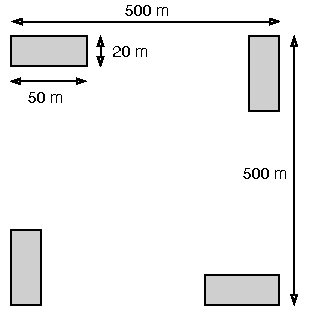
\includegraphics[width=0.5\textwidth]{schematic}
	\caption{Schematic diagram of plot layout within a site. Each 20$\times$50
		m (0.1 ha) plot is shaded grey. Note that the plot dimensions are not to
		scale.}
	\label{schematic}
\end{figure}

Within each plot, the species and basal area of all trees with at least one
stem $\geq$\stemSize{} cm DBH were recorded. Plot data were aggregated to the
site level for all analyses to avoid pseudo-replication. Each site spans an
area 500$\times$500 m (0.25 km\textsuperscript{2}), matching that of the land
surface phenology data. We excluded sites where plots differed appreciably in
vegetation composition, to ensure that all sites used in statistical analysis
were representative of the vegetation within the total 0.25
km\textsuperscript{2} area of each site. Using the Bray-Curtis dissimilarity
index on species basal area data \citep{Faith1987}, we calculated the mean
pairwise compositional distance between plots within each site. Sites were
discarded when the mean pairwise compositional distance among plots within the
site was greater than the mean pairwise compositional distance of all plots
across all sites. This resulted in a final dataset of \plotDistN{} sites.

\subsection{Vegetation composition and diversity} 

To describe variation in tree species composition across sites we used
agglomerative hierarchical clustering on species basal area data
\citep{Kreft2010, Fayolle2014} to assign sites to vegetation types. We excluded
species with fewer than five records across all sites from this analysis, as
very rare species can hinder meaningful cluster delineation. We used Ward's
algorithm to define clusters \citep{Murtagh2014}, based on the Bray-Curtis
distance between pairs of sites. We determined the optimal number of clusters
by maximising the mean silhouette width among clusters \citep{Rousseeuw1987}.
We described the vegetation types represented by each cluster using
Dufr\^{e}ne-Legendre indicator species analysis \citep{Dufrene1997}, which
ranks species as the product of their relative frequency and their relative
average abundance in each vegetation type. \Numberstringnum{\nCluster}
vegetation types were identified during hierarchical clustering. The mean
silhouette value of the clustering algorithm was \silBest{}. 

There was some spatial and climatic stratification in vegetation composition
(\autoref{site_map}). Three miombo woodland types were identified, each with
different sets of secondary species, but all dominated by detarioid species
such as \textit{Brachystegia} spp. and \textit{Julbernardia} spp.
(\autoref{clust_summ}). Uapaca miombo is largely absent from the southwest of
the country, occurring predominantly in higher rainfall regions to the north
and east (\autoref{box_facet_map_mat}). Cryptosepalum miombo is found more in
the southwest of the country, possibly representing the drier ``Angolan miombo
woodlands'' described by \citet{White1983}. While Cryptosepalum miombo
woodlands include \textit{Cryptosepalum exfoliatum} as a secondary species,
they should not be confused with Zambezian evergreen forests, which are
dominated by Cryptosepalum \citep{White1983}. Julbernardia miombo is common in
cooler areas and is more climatically restricted than the other miombo woodland
types. Combretaceae woodlands match the description of small stature Zambezian
woodlands, as described by \citet{Dinerstein2017} and \citet{Chidumayo2001}.
These woodlands are not dominated by the same archetypal detarioid tree species
as the other miombo woodland vegetation types. These Combretaceae woodlands
occur over a wide climatic range, and contain some of the warmest sites in our
dataset in the southeast of the country. \DIFdelbegin \DIFdel{The miombo woodland vegetation types
are dominated by }\textit{\DIFdel{Brachystegia}} %DIFAUXCMD
\DIFdel{spp. and }\textit{\DIFdel{Julbernardia}} %DIFAUXCMD
\DIFdel{spp.,
with different secondary species. }\DIFdelend Median species richness and the range of
species richness values per site is similar across vegetation types
(\autoref{clust_summ}). 

\begin{figure}[H]
\centering
	\includegraphics[width=\textwidth]{site_map}
	\caption{Distribution of study sites, within Zambia (left), and in climate
		space (right). Sites are shown as triangles, coloured according to
		vegetation type. Zambia is shaded according to mean growing season length
		during the period \modisStart{} to \modisEnd{}, estimated from the MODIS
		MCD12Q2 land surface phenology product, at 500 m spatial resolution
		\citep{MCD12Q2}. Growing season length is masked by the MODIS MCD12Q1 land
		cover map from 2015 \citep{MCD12Q1}, removing all pixels occurring in wetlands,
		croplands, water bodies, and urban areas. Climate space is represented by Mean
		Annual Temperature (MAT) and Mean Annual Precipitation (MAP), extracted from
		the WorldClim dataset at 30 arc second resolution \citep{Fick2017}. The shaded
		area in the right panel shows the climate space of Zambia, showing the density
		of pixels for given values of MAT and MAP. The ellipses in the right panel show
		the 95th percentiles of the climate space of each vegetation type.} 
	\label{site_map}
\end{figure}

\setlength{\tabcolsep}{2pt} % Default table column sep width 
\input{out/clust_summ.tex}
\setlength{\tabcolsep}{4pt} % Default table column sep width 

\begin{figure}[H]
\centering
	\includegraphics[width=\textwidth]{box_facet_map_mat}
	\caption{Mean Annual Precipitation and Mean Annual Temperature for each
		site, grouped by vegetation type. Climate data were extracted from the
	    WorldClim dataset at 30 arc second resolution \citep{Fick2017}.} 
	\label{box_facet_map_mat}
\end{figure}

To describe species diversity in each site, we calculated the Shannon-Wiener
index ($H'$) from species basal area rather than individual abundance, as a
measure of species diversity effectively weighted by a species' contribution to
canopy occupancy and thus the land surface phenological signal. $H'$ was
transformed to the first-order numbers-equivalent ($^1\!D$) of $H'$, calculated
as $e^{H'}$, which gives the equivalent number of equally common species that
would result in a given value of $H'$, also known as effective species richness
\citep{Jost2007}. We use $^1\!D$ as the primary measure of species diversity in
our statistical models, and is subsequently referred to as species diversity.
To describe \DIFaddbegin \DIFadd{the abundance of Detarioid species we calculated their proportional
basal area. To describe }\DIFaddend average tree size, we calculated the
quadratic mean of stem diameters per site. Quadratic mean diameter is exactly
related to site basal area, unlike the arithmetic mean of diameter, and assigns
greater weight to larger trees \citep{Curtis2000}. It is thus a more
appropriate descriptor of average stem size for this study, where the
arithmetic mean would be biased by an abundance of small stems, despite their
small contribution to overall canopy land surface phenological signal. 

\subsection{Remote sensing data}

Precipitation time series data for each site was compiled from the GPM IMERG
Final Precipitation L3 1 day V06 product, which has a pixel size of
0.1\textdegree (11.1 km at the equator) \citep{IMERG}. We used all available
data from \modisStart{} to \modisEnd{}. There is no clear consensus on best
practice for defining the limits of the rainy season \citep{Guan2014}. Here we
followed the example of \citet{Stern1981} and \citet{Adole2018a}, variations of
which have been used in other studies of African savanna-woodland phenology
\citep{Mupangwa2011, Segele2005}. First, we determined the temporal bounds of
each wet-dry season cycle within our study period of \modisStart{} to
\modisEnd{} for each site according to \citet{Ferijal2022}, as the 14 day
period with the lowest precipitation in each calendar year. Where multiple 14
day periods tied for lowest precipitation within a single calendar year, the
later period was chosen. 

The onset of the rainy season for each wet-dry season cycle was defined as the
start of the first period of \onsetPeriodOne{} days with more than
\onsetPrecipOne{} mm total rainfall, immediately followed by \onsetPeriodTwo{}
days with more than \onsetPrecipTwo{} mm total rainfall \citep{Tadross2005}. With this rolling
window approach we sought to identify the first sustained period where \DIFdelbegin \DIFdel{tree
}\DIFdelend \DIFaddbegin \DIFadd{plant
}\DIFaddend available soil moisture was increasing, i.e. where the average regional
evaporation rate of \textasciitilde{}1 mm per day was exceeded by rainfall
\citep{Campbell1996}, while accounting for the stochastic nature of rainfall in
our study at the start of the rainy season. We chose to relax the rainfall
constraint from \DIFdelbegin %DIFDELCMD < \onsetPrecipOne{} %%%
\DIFdel{mm to }%DIFDELCMD < \onsetPrecipTwo{} %%%
\DIFdel{mm }\DIFdelend \DIFaddbegin \DIFadd{2 mm d\textsuperscript{-1} in the first 10 day period, to 1 mm d\textsuperscript{-1} }\DIFaddend for the subsequent
20 day period\DIFaddbegin \DIFadd{, }\DIFaddend to account for variation in the temporal consistency of rainfall
at the start of the rainy season in our study region. As opposed to a
percentile of cumulative rainfall approach, our method is not affected by dry
season storm-burst rainfall events, which, while contributing to overall
cumulative rainfall, often do not have the capacity to initiate tree foliage
production due to their transience \citep{February2016}. 

The end of the rainy season was defined as the start of the first period where
fewer than \numberstringnum{\rainyDaysEnd} days within a \periodEnd{} day
period received more than \rainyDef{} mm rainfall. \citet{Guan2014} compares
other methods of estimating rainy season onset and end dates, and finds little
functional difference between the method chosen here and other common methods.
To validate our \DIFdelbegin \DIFdel{chosen definition of }\DIFdelend \DIFaddbegin \DIFadd{delimitation of the }\DIFaddend rainy season we checked that all season
start and end dates occurred within 10 days of the dates where 10\% and 95\% of
yearly cumulative rainfall were \DIFdelbegin \DIFdel{exceeded, for each wet-dry season cycle
}\DIFdelend \DIFaddbegin \DIFadd{surpassed, respectively }\DIFaddend \citep{Adole2018a}. 

To quantify seasonal patterns of leaf display at each site, we used the MODIS
MCD12Q2 v6.1 land surface phenology product \citep{MCD12Q2}. MCD12Q2 provides
annual metrics describing land surface phenology, with a spatial resolution of
\textasciitilde{}500 m. The phenological metrics in MCD12Q2 are derived from
the \DIFdelbegin \DIFdel{EVI2 (}\DIFdelend 2-band Enhanced Vegetation Index \DIFdelbegin \DIFdel{) }\DIFdelend time series (1-2 day temporal resolution), with nadir Bidirectional Reflectance
Distribution Function-adjusted surface reflectance \DIFaddbegin \DIFadd{(NBAR-EVI2)}\DIFaddend . There are a number of land
surface phenology products derived from MODIS vegetation indices. MCD12Q2 was
chosen here as it has been used effectively in other studies in deciduous
African woodlands to define the growing season \citep{Begue2014, Adole2018b}.
Additionally, a previous comparison of MODIS-derived land surface phenology
products showed that MCD12Q2 out-performed other products in predicting the
start of the growing season in relation to ground observations
\citep{Peng2017}. 

All sites were determined to have a single annual growing season according to
the MCD12Q2 ``NumCycles'' metric. We used all years of data from \modisStart{}
to \modisEnd{}. We used the ``Greenup'' and ``Dormancy'' metrics to define the
growing season as the period when the EVI time series exceeds 15\% of the EVI
amplitude for a given growing season (\autoref{ts_illus}). We used the
``Maturity'' \DIFdelbegin \DIFdel{metric }\DIFdelend \DIFaddbegin \DIFadd{and ``Senescence'' metrics, defined as the dates bounding the
period where the EVI time series exceeds 90\% of the EVI amplitude, }\DIFaddend to define
the end of the green-up period \DIFdelbegin \DIFdel{, and the ``Senescence'' metric to define the }\DIFdelend \DIFaddbegin \DIFadd{and the }\DIFaddend start of the senescence period\DIFaddbegin \DIFadd{,
respectively}\DIFaddend . We used these dates to calculate the length of the green-up
period and senescence period. We calculated ``pre-rain green-up'' as the number
of days between the onset of the growing season and the onset of the rainy
season, for each year of available data. Similarly we calculated ``senescence
lag'' as the number of days between the end of the rainy season and the end of
the growing season. To aid interpretation of statistical models, we reversed
the sign of the pre-rain green-up measurements, so that larger values indicate
earlier pre-rain green-up. As senescence generally occurred after the end of
the rainy season, we did not reverse the sign of senescence lag, so larger
values indicate later senescence\DIFdelbegin \DIFdel{lag}\DIFdelend . 

Daily total precipitation from the GPM IMERG product was separated into three
periods of relevance to different phenological metrics: precipitation during
the growing season, precipitation in the 30 day period before the onset of the
growing season (pre-green-up precipitation), and precipitation in the 30 day
period before the onset of senescence at the end of the growing season
(pre-senescence precipitation) \DIFaddbegin \DIFadd{(}\autoref{ts_illus}\DIFadd{)}\DIFaddend . 

Temperature time series data for each site was compiled from the ERA5-Land
hourly data, using the 2 m air temperature variable at 0.1\textdegree (11.1 km
at the equator) \citep{ERA5}. We aggregated these data to the maximum
temperature for each day over the period \modisStart{} to \modisEnd{}. We then
calculated cumulative temperature during the 30 day pre-green-up period, 30 day
pre-senescence period, and the growing season period, as with the precipitation
data. Cumulative temperature has been shown in previous studies to be an
important cue driving patterns of leaf display in more temperate systems
\citep{Archibald2007, Michelson2017, Escamilla2020}. While the spatial scales
of the climate data (0.1\textdegree{}) and land surface phenology data (500 m)
do not match we believe this does not present a problem for our analyses.
Firstly, because temperature and rainfall data are expressed in our analyses as
cumulative values across longer time periods, \DIFdelbegin \DIFdel{e.g. cumulative rainfall }\DIFdelend \DIFaddbegin \DIFadd{for example cumulative rainfall over the }\DIFaddend 30 days
prior to green-up, we do not expect systematic spatial variation in these
aggregated values within each 0.1\textdegree{} pixel, especially when
considering multiple years of data. Secondly, the distance among sites is much
greater than the resolution of the climate data. Any variation in temperature
or rainfall within pixels is likely to be less than that among sites.

\begin{figure}[H]
\centering
	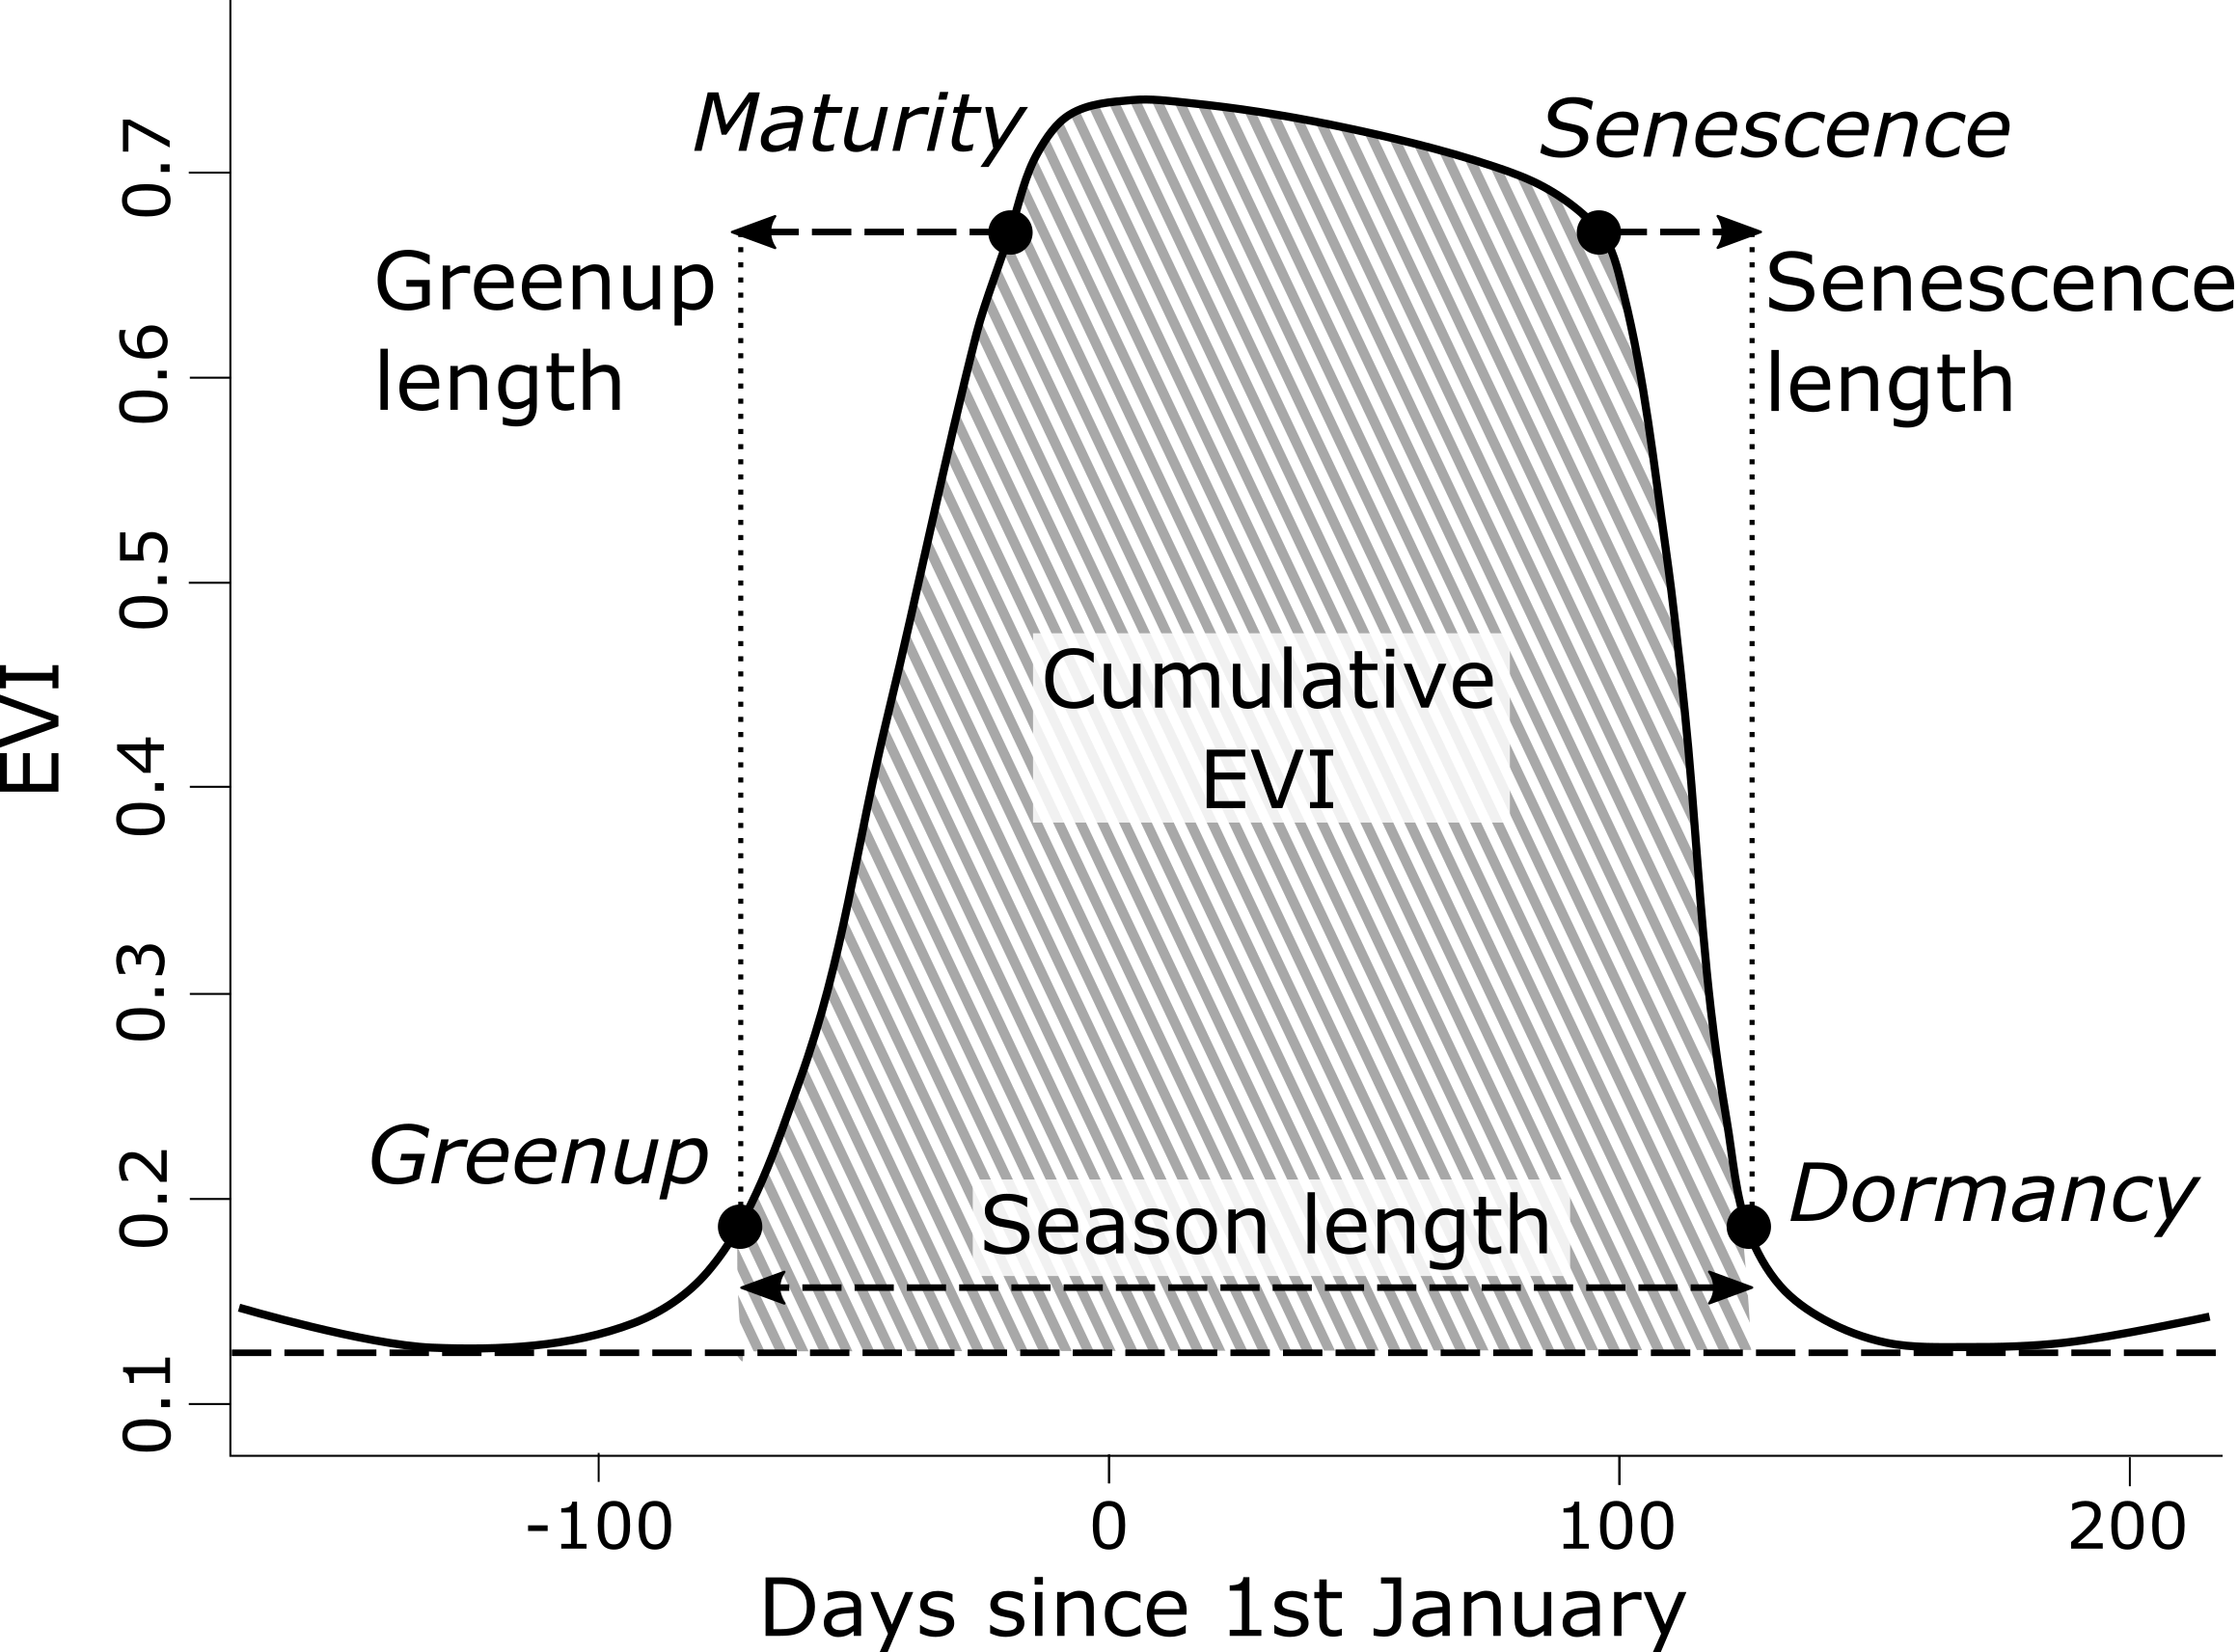
\includegraphics[width=0.8\textwidth]{ts_illus}
	\caption{Schematic diagram of hypothetical splined NBAR-EVI2 time series
		(black curve), from which metrics provided by the MCD12Q2 product are
		derived (black circles). Cumulative EVI is denoted by the shaded area under the EVI
		curve for a given growing season, bounded by the ``Greenup'' and ``Dormancy''
		dates. The blue curve shows a hypothetical splined 10 day rolling total
		rainfall time series, derived from the GPM IMERG product. Blue circles indicate
		the start and end of the rainy season as defined by our algorithm. Dashed black
		lines indicate the derived phenological metrics used in this study. In this
		hypothetical example, ``Greenup'' occurs in advance of the start of the rainy
		season, and ``Dormancy'' occurs after the end of the rainy season, reflecting
		the condition of \posGrePer{}\% (\posGre{}/\nTable{}) of the yearly data in our
		dataset. In \posSenPer{}\% (\posSen{}/\nTable{}) of cases, dormancy occurred
		after the end of the rainy season and green-up occurred after the start of the
		rainy season. In \negSenPer{}\% (\negSen{}/\nTable{}) of cases, dormancy
		occurred before the end of the rainy season. Adapted from \citet{Gray2022}.}
	\label{ts_illus}
\end{figure}

\subsubsection{Statistical modelling}

Linear mixed effects models were used to investigate the effect of tree species
diversity \DIFaddbegin \DIFadd{(effective number of species)}\DIFaddend , species composition \DIFaddbegin \DIFadd{(relative
abundance of Detarioid species)}\DIFaddend , and woodland structure \DIFaddbegin \DIFadd{(quadratic mean of stem
diameter) }\DIFaddend on each of the six phenological metrics \DIFaddbegin \DIFadd{(cumulative EVI, season
length, length of green-up period, length of senescence period, pre-rain
green-up, senescence lag)}\DIFaddend . We specified a maximal model structure including the
fixed effects of species diversity, mean tree stem diameter, relative abundance
of detarioid species, precipitation and cumulative temperature, the latter two
of which have been shown by previous studies to strongly influence patterns of
foliage display, including green-up and senescence \citep{Whitecross2017,
Adole2019}. For models of growing season length and cumulative EVI we used
total cumulative rainy season precipitation and total cumulative rainy season
temperature; for pre-rain green-up and length of green-up period we used
pre-green-up precipitation and cumulative temperature; for senescence lag and
length of senescence period we used pre-senescence precipitation and cumulative
temperature. All models included a random intercept term for site to account
for yearly repeated measurements of site land surface phenology. Fixed effects
in each model were standardised to Z-scores prior to modelling to allow
comparison of slope coefficients within models. 

To determine the magnitude and direction of each fixed effect on each
phenological metric, we compared standardised effect sizes extracted from
models re-estimated using Maximum Likelihood. For each fixed effect we
calculated the 95\% confidence interval of the effect size as 1.96$\times{}$
the standard error of the parameter estimate \citep{Zuur2010}. All statistical
analyses were conducted in R version 4.0.2 \citep{R2020}.

\section{Results}

The majority of sites experienced pre-rain green-up, with the site mean date of
green-up occurring in advance of the onset of the rainy season in
\posGreAll{}/\nSites{} sites. Across all sites, the mean lag between green-up
and the onset of seasonal rains was \greenLagMean{} days ($\pm{}$1 standard
deviation). Linear mixed effects models effectively explained 
pre-rain green-up (R\textsuperscript{2}\textsubscript{m}=\glagRm{},
R\textsuperscript{2}\textsubscript{c}=\glagRc{}), 
cumulative EVI (R\textsuperscript{2}\textsubscript{m}=\cumviRm{},
R\textsuperscript{2}\textsubscript{c}=\cumviRc{}), 
green-up length (R\textsuperscript{2}\textsubscript{m}=\grateRm{},
R\textsuperscript{2}\textsubscript{c}=\grateRc{}) and 
season length (R\textsuperscript{2}\textsubscript{m}=\lengthRm{},
R\textsuperscript{2}\textsubscript{c}=\lengthRc{}), while 
senescence length (R\textsuperscript{2}\textsubscript{m}=\srateRm{},
R\textsuperscript{2}\textsubscript{c}=\srateRc{}) and 
senescence lag (R\textsuperscript{2}\textsubscript{m}=\slagRm{},
R\textsuperscript{2}\textsubscript{c}=\slagRc{}), were poorly explained. Fixed
effects explained the majority of total variance explained in models for
pre-rain green-up, season length and green-up length, while the random effect
of site explained most of the variance in cumulative EVI (\autoref{modtab}).

We compared standardised effect sizes of fixed effects for each phenological
metric to determine the strength and direction of their influence
(\autoref{mod_slopes}). Tree species diversity exhibited positive
effects on season length (\slRich{}, standardised coefficient $\pm$1 standard
error) (H\textsubscript{1}) and pre-rain green-up (\prRich{})
(H\textsubscript{2}). Average tree size, measured by the quadratic mean of stem
DBH per site, was a significant predictor of pre-rain green-up (\prSize{}) and
green-up length (\glSize{}), associated with early pre-rain green-up and a
longer green-up period (H\textsubscript{3}). Sites with larger trees also
experienced later senescence (\slSize{}). The proportional basal area 
\DIFdelbegin \DIFdel{abundance
}\DIFdelend of detarioid species was a significant predictor of pre-rain green-up
(\prDet{}), and season length (\slDet{}) (H\textsubscript{4}). 

\begin{figure}[H]
\centering
	\includegraphics[width=\textwidth]{mod_slopes_all.pdf}
	\caption{Standardised fixed effect coefficients (dots) with 95\% confidence
		intervals (whiskers) for models of each phenological metric (panels). Estimates where the 95\% confidence interval does not overlap zero are
		considered to be significant and are marked by asterisks. \DIFaddbeginFL \DIFaddFL{Degree days and precipitation data were summed over different periods most relevant to each phenological metric. Green-up length and pre-rain green-up used data from the 30 day pre-green-up period, senescence length and senescence lag used data from the 30 day pre-senescence period, cumulative EVI and season length used data from the growing season period.}\DIFaddendFL }
	\label{mod_slopes}
\end{figure}

\section{Discussion}

We have demonstrated clear effects of tree species diversity, composition and
structure on various metrics of land surface phenology in deciduous woodlands
across Zambia. Both tree species diversity and the basal area \DIFdelbegin \DIFdel{abundance }\DIFdelend of
trees from the Detarioideae (subfamily of Fabaceae), were associated with a
longer growing season and with earlier pre-rain green-up. Our models partition
the effects of species diversity and detarioid abundance, suggesting that while
some of the positive species diversity effect is due to niche complementarity,
i.e. a true diversity effect, some is due to the increased likelihood of
containing species able to green-up earlier, i.e. a mass-ratio effect
\citep{Grime1998, Tilman2014}. Our study lends support for a general positive
effect of tree species diversity on ecosystem function in southern African
deciduous woodlands, measured through leaf display \citep{Richardson2009},
which aligns with other recent studies in the region \citep{Godlee2021,
McNicol2018, Shirima2015}. Additionally, our results highlight the \DIFdelbegin \DIFdel{keystone }\DIFdelend \DIFaddbegin \DIFadd{important
}\DIFaddend role of detarioid species in southern African \DIFdelbegin \DIFdel{woodlands, affecting ecosystem structure, the wildlife provisioning role, and
productivity}\DIFdelend \DIFaddbegin \DIFadd{woodland productivity: we show
that increasing abundance of these species increases both early season
productivity and overall growing season length}\DIFaddend .

The basal area \DIFdelbegin \DIFdel{abundance }\DIFdelend of detarioid species had a positive effect on pre-rain green-up.
Our results suggest a mass-ratio effect in the pre-rain green-up of Zambian
deciduous woodlands \citep{Grime1998}, whereby a dominant functional group of
trees with particular traits and life history strategy, \DIFdelbegin \DIFdel{are }\DIFdelend \DIFaddbegin \DIFadd{is }\DIFaddend able to green-up in
advance of seasonal rains \DIFdelbegin \DIFdel{, }\DIFdelend \DIFaddbegin \DIFadd{and }\DIFaddend drive longer growing seasons\DIFdelbegin \DIFdel{, and
overall drive greater productivity}\DIFdelend . Given their
tendency to create deep root networks which provide effective water and
non-structural carbohydrate storage \citep{Zhou2020, Timberlake1993}, and their
high wood density which confers embolism-resistance to the tree hydraulic
system \citep{Hoffmann2011, Hacke2001, Chave2009}, we suggest that compared to
other co-occurring taxonomic groups, detarioid species are better equipped to
green-up before seasonal rainfall begins \citep{Vinya2018}. In our analysis we
accounted for the effect of tree size on pre-rain green-up, which generally
correlates with rooting depth, and still found an effect of detarioid abundance
on pre-rain green-up, implying a true effect of detarioid species not linked to
tree size. While pre-rain green-up is a risky strategy, it may provide a
competitive advantage for detarioid species, allowing them to take advantage of
early rainfall and associated soil nutrient release \citep{February2016}.

While at present the ability to green-up prior to the rainy season provides a
competitive advantage to detarioid species by extending the period of
productivity, it is unclear whether this behaviour will continue to provide a
benefit under a changing climate, where the timing of the rainy season is
expected to shift\DIFdelbegin \DIFdel{in time, become shorter, and become more erratic }\DIFdelend \DIFaddbegin \DIFadd{, becoming more erratic and shorter overall
}\DIFaddend \citep{Shongwe2011, Pohl2017, Wainwright2021}. Given the dominance of detarioid
species in miombo woodlands across southern Africa, decreased productivity of
this group due to a mismatch between leaf display and seasonal rainfall may
affect the future composition, structure and functioning of these woodlands,
potentially leading to a shorter stature, lower biomass and lower productivity
ecosystem.

Environmental variables had consistently strong effects on phenological
metrics, and confirm previous research. Greater rainfall within the rainy
season led to a longer growing season and greater cumulative EVI, matching our
expectations that increased water availability allows for greater foliage
production and builds groundwater reserves allowing for a longer growing season
\citep{Adole2018a}. Surprisingly, greater rainfall in the 30 days leading up to
the start of the growing season was associated with later green-up with respect
to the onset of the rainy season. We suggest this may be the result of large
amounts of rainfall kick-starting foliage production in the absence of a
pre-rain green-up effect in some sites, and may represent cases where grasses
drive the start of growing season land surface phenology signal. This inability
to discriminate between the grassy component and the tree canopy component of
the phenological signal highlights one of the principle drawbacks with
space-borne land surface phenology to characterise patterns of vegetation leaf
display \citep{Archibald2007}. Hotter days were associated with shorter periods
of senescence and green-up\DIFaddbegin \DIFadd{, but ultimately a longer growing season and greater
overall productivity}\DIFaddend . In the case of green-up length, this effect may imply a
temperature trigger on leaf display, as is seen in temperate woodland
ecosystems \citep{Flynn2018}. In the case of senescence, hotter days \DIFaddbegin \DIFadd{at the end
of the growing season }\DIFaddend are expected to increase photorespiration and ultimately
result in a negative leaf carbon balance, triggering leaf loss
\citep{Warren2011, Marin2019}. This study provides a glimpse into how climate
change, particularly warming \citep{IPCC} and increased rainfall seasonality
\citep{Wainwright2021}, could \DIFdelbegin \DIFdel{strongly
}\DIFdelend affect leaf phenology in the future in southern
Africa. \DIFdelbegin \DIFdel{Increased temperature and decreased precipitation were both strongly associated with decreased
growing season length, and
weakened the pre-rain }\DIFdelend \DIFaddbegin \DIFadd{Future temperature increases in miombo woodlands, particularly high
temperatures at the start and end of the rainy season, could
accelerate }\DIFaddend green-up \DIFdelbegin \DIFdel{effect}\DIFdelend \DIFaddbegin \DIFadd{and senescence processes. Similarly, a reduction in
precipitation during the growing season could reduce growing season length and
overall productivity}\DIFaddend . Future studies could explore further how climate extremes
affect land surface phenology, ideally in combination with measurements of
\DIFdelbegin \DIFdel{composition and
}\DIFdelend \DIFaddbegin \DIFadd{species composition and ecosystem }\DIFaddend structure, which \DIFdelbegin \DIFdel{we expect from this study might mediate the effect of climate
extremes}\DIFdelend \DIFaddbegin \DIFadd{this study has shown are
also important drivers of ecosystem function}\DIFaddend .

The end of the growing season came later with respect to the end of the rainy
season in plots with larger mean stem diameter, though our model had low
explanatory power. \citet{Cho2017} found that tree cover, measured by MODIS
Leaf Area Index (LAI) data, had a significant positive effect on end of growing
season date in tropical dry woodlands in South Africa. Similarly,
\citet{Guan2014} found at continental scale across Africa that the end of the
growing season came later with respect to the end of the rainy season in areas
where tree cover was higher. Both these previous studies posit that the
observed effect of tree cover on end of growing season date might indicate the
presence of larger trees capable of accessing deeper groundwater reserves or
holding stem-water reserves after the rainy season ends and surface soil
moisture is depleted. Our study lends further support for this suggestion by
directly testing the effect of tree size, rather than tree cover. 

Our best models predicting the length of the senescence period and the end of
growing season lag did not explain much of the variance in these phenological
metrics. Short term oscillations in soil moisture driven by localised rainfall
events, and the condition of ground cover vegetation may be responsible for
driving the length of the senescence period, hence the wide variability of this
phenological metric and the poor fit of our statistical models. Most of the
variance explained by our models of senescence period length and senescence lag
came from the random effect of site, implying some unmeasured inter-site
variation. Grass productivity is more reactive to short-term changes in soil
moisture than tree activity, and may oscillate within the senescence period
\citep{Archibald2007}. This may explain the lack of a strong growing season
precipitation or tree diversity signal for senescence lag and length of the
senescence period in our models.

Other studies, both globally and within southern African woodlands, have
largely ignored patterns of senescence, instead focussing on patterns of
green-up \citep{Gallinat2015}. Most commonly, studies of senescence simply
correlate the decline of rainfall with senescence \citep{Stevens2016,
Guan2014}, but our best model suggests that temperature is a stronger
determinant of the end of the growing season than precipitation. We suggest
that hotter days \DIFdelbegin \DIFdel{in the period leading up to the start of the senescence period }\DIFdelend \DIFaddbegin \DIFadd{at the end of the growing season }\DIFaddend might accelerate senescence
through tissue damage and embolism \citep{Cho2017}, resulting in a shorter
\DIFdelbegin \DIFdel{senescence period length}\DIFdelend \DIFaddbegin \DIFadd{period of senescence}\DIFaddend . In temperate ecosystems, which experience autumn
senescence, lower night time temperatures have been shown to increase the rate
of senescence and thus decrease senescence period length \citep{Michelson2017,
Escamilla2020}. In these water-limited and hot systems however, it seems hotter
temperatures are the main driver \DIFdelbegin \DIFdel{. Similarly, hotter
}\DIFdelend \DIFaddbegin \DIFadd{of senescence. Hotter }\DIFaddend days prior
to senescence appear to \DIFdelbegin \DIFdel{advance }\DIFdelend \DIFaddbegin \DIFadd{delay }\DIFaddend the onset of senescence with respect to the end
of the rainy season, \DIFdelbegin \DIFdel{possibly due to increased evaporative demand
and increased photorespiration, which might trigger leaf loss, in response to
an increasingly negative carbon balance. These suggestions however, must be
considered in the context that the fixed effects in our models did not account
for much of the variation in senescence period length or senescence lag}\DIFdelend \DIFaddbegin \DIFadd{and higher temperatures across the growing season were
associated with a longer growing season. Thus, while climate warming could
accelerate the process of senescence, it may also delay the senescence period with respect
to the end of the rainy season}\DIFaddend .

Alternatively, \citet{Zani2020} suggests that in resource-limited environments,
senescence times may largely be set by the preceding photosynthetic activity
and sink-limitations on growth. For example, limited nutrient supply may
prohibit photosynthesis late in the season if the preceding photosynthetic
activity has depleted that supply. \citet{Reich1992} suggested that there are
many direct constraints on leaf life-span such as drought and herbivory,
especially in the seasonally dry tropics, which would lead to timing of
senescence being set largely by the time of bud-burst. Our study indirectly
corroborates this theory, with the finding of a moderate negative correlation
between pre-rain green-up and senescence lag across all vegetation types
indicating that later green-up allows later senescence (\autoref{phen_bivar}).

We found positive effects of mean tree size (site quadratic mean diameter) on
pre-rain green-up and green-up length, but negative effects on senescence lag.
Our results agree with previous studies that the increased rooting depth of
large trees allows them to access deep ground-water reserves, conferring
resilience to inter-annual variation in patterns of seasonal rainfall
\citep{Holdo2017}. While detarioid species in these woodlands tend to grow to
large sizes, our result of a significant effect of tree size alongside an
effect of detarioid abundance on pre-rain green-up infers particular traits
beyond tree size in the detarioid species that drive pre-rain green-up.

Our finding that species diversity increases growing season length and
cumulative EVI in seasonally dry tropical woodlands provides an example of a
mechanism by which species diversity increases ecosystem function, a pattern
observed previously in other studies of southern African woodlands
\citep{Godlee2021, McNicol2018, Shirima2015}, and globally in other biomes
\citep{Plas2019, Tilman2014}. Our findings provide earth system modellers with
an insight to better understand how changes in the inter-related variables of
species diversity, composition and structure affect \DIFaddbegin \DIFadd{one measure of ecosystem
function (}\DIFaddend land surface phenology\DIFaddbegin \DIFadd{)}\DIFaddend . Future studies should aim to disentangle
these effects further, possibly in an experimental context. Incorporating
predictions of biotic composition and its change over time into earth system
models has been limited until recently for two main reasons\DIFdelbegin %DIFDELCMD < \citep{Ahlstrom2015, Bodegom2011}%%%
\DIFdelend . Firstly, there are
large uncertainties in the effects of biodiversity on ecosystem function, e.g.
gross primary productivity (GPP) \DIFaddbegin \citep{Ahlstrom2015}\DIFaddend . Secondly, until recently
there has been a major paucity of ground data on community composition, and a
lack of appropriate remote-sensing data to scale up to larger areas
\DIFaddbegin \citep{Bodegom2011}\DIFaddend . Our study comes at a pertinent time \DIFdelbegin \DIFdel{when }\DIFdelend \DIFaddbegin \DIFadd{where }\DIFaddend plot-based
vegetation monitoring networks \DIFdelbegin \DIFdel{have become sufficiently widespread }\DIFdelend \DIFaddbegin \DIFadd{are now sufficiently widespread to robustly test
hypotheses and generate theory on the effects of community composition on
ecosystem function across environmental gradients }\DIFaddend \citep{ForestPlotsnet2021,
SEOSAW2020}\DIFdelbegin \DIFdel{, and remotely sensed proxies
of diversity in forested ecosystems are becoming sophisticated enough
}%DIFDELCMD < \citep{Schneider2017, Cavendar2020} %%%
\DIFdel{to be of
real use to
}\DIFdelend \DIFaddbegin \DIFadd{. Additionally, recent advances in remote sensing of functional
diversity from hyper-spectral data, combined with the imminent deployment of
space-borne imaging spectrometers by multiple space agencies
}\citep{CawseNicholson2021, Rast2021}\DIFadd{, will soon allow community composition to
be mapped at large spatial scales }\citep{Wallis2024, Cavendar2020} \DIFadd{and utilised
by }\DIFaddend earth system modellers. Our study \DIFdelbegin \DIFdel{provides a link by demonstrating a strong relationship
between species diversity and land surface phenology, particularly growing
season length, which is itself closely correlated with GPP
}%DIFDELCMD < \citep{Sjostrom2011}%%%
\DIFdelend \DIFaddbegin \DIFadd{serves as an example of the kinds of
advancements in ecological understanding relevant to earth system modelling
that can be made by integrating abundant ground data and remote sensing data}\DIFaddend .

\section{Conclusion}

We explored how tree species diversity, composition and structure of deciduous
woodlands influence land surface phenology across Zambia. We showed that
species diversity drives longer growing seasons and promotes earlier pre-rain
green-up across woodlands in the miombo ecoregion. The abundance of
Detarioideae species (subfamily of Fabaceae) had a consistent positive effect
on pre-rain green-up and over-all growing season length, supporting suggestions
from previous studies of their \DIFdelbegin \DIFdel{keystone }\DIFdelend \DIFaddbegin \DIFadd{important }\DIFaddend role in driving pre-rain green-up in
southern African miombo woodlands. Finally, we found that larger trees drive
earlier pre-rain green-up supporting previous research suggesting that deep
roots and persistent carbohydrate storage allows for precocious leaf display.

Our results lend further support to an already well established corpus of study
on the positive effect of species diversity on ecosystem function.
Additionally, our results provide evidence for earth-system modellers,
demonstrating the importance of structure and diversity in determining patterns
of land surface phenology. As reliable data on ecosystem structure\DIFaddbegin \DIFadd{,
particularly tree size, }\DIFaddend become available across larger spatial scales and at
higher spatial resolution, we hope that these data can be explored in models of
land-atmosphere mass and energy exchange to improve their predictive skill
under a changing climate.

\printbibliography

\section{Supplementary Material}
\beginsupplement

\begin{figure}[H]
\centering
	\includegraphics[width=\textwidth]{phen_bivar}
	\caption{Scatter plots showing pairwise comparisons of the six phenological
		metrics used in this study, extracted from the MODIS MCD12Q2 product
		\citep{MCD12Q2}. Points represent study sites and are coloured by vegetation
		type. Linear regression line of best fit for all sites is shown as a black
		line, while linear regressions are shown for each vegetation type as coloured
		lines. Non-significant linear regression fits (p<0.05) have dashed lines. The
		units of `d' are the number of days.}
	\label{phen_bivar}
\end{figure}

\begin{landscape}
\input{out/modtab_adj.tex}
\end{landscape}

\end{document}

